
%(BEGIN_QUESTION)
% Copyright 2012, Tony R. Kuphaldt, released under the Creative Commons Attribution License (v 1.0)
% This means you may do almost anything with this work of mine, so long as you give me proper credit

Hydrokrakkingsprosessen i raffineri er eksoterm. Temperatur i reaktor styres ved tilsetting av hydrogen som ``quench''. Tre identiske temperaturtransmittere måler samme punkt, og signalene går via medianvelger (TY-24) til regulatoren:

$$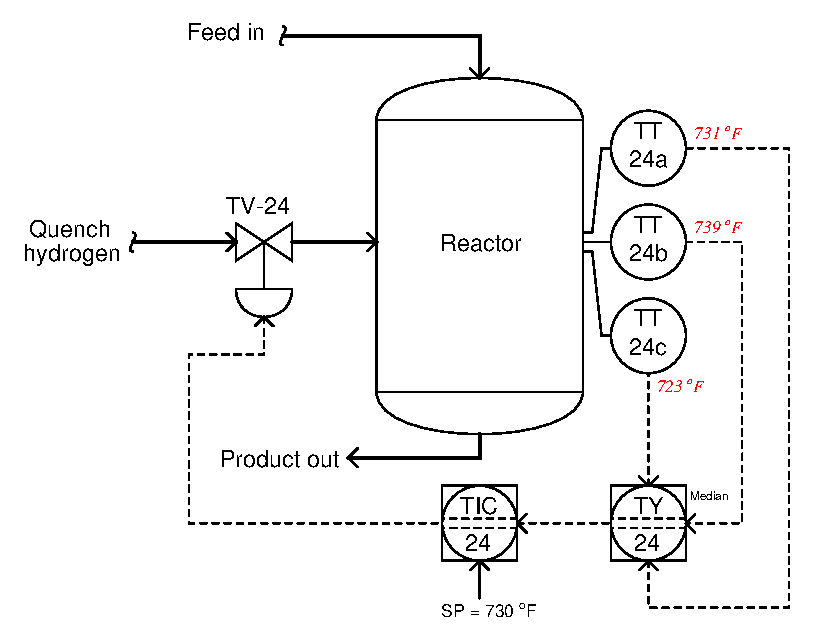
\includegraphics[width=15.5cm]{i00972x01.eps}$$

\noindent
Velg beste svar for umiddelbar effekt dersom TT-24b plutselig feiler med {\it høyt} signal:

\begin{itemize}
\item{} Quench-hydrogenventil (TV-24) lukker litt for å øke temperatur
\vskip 10pt
\item{} Quench-hydrogenventil (TV-24) åpner kraftig for å senke temperatur
\vskip 10pt
\item{} Ingenting skjer. TV-24 holder samme posisjon
\vskip 10pt
\item{} TV-24 åpner litt for å senke temperatur
\end{itemize}


\underbar{file i00972}
%(END_QUESTION)





%(BEGIN_ANSWER)

Ingenting skjer. Quench-hydrogenventilen (TV-24) holder samme posisjon.
 
%(END_ANSWER)





%(BEGIN_NOTES)

{\bf Denne oppgaven er ment kun for eksamen, ikke for arbeidsark!}.

%(END_NOTES)

